\chapter{Evolutionary Algorithm Configuration} % (fold)
\label{cha:evolutionary_algorithm_configuration}

\section{Background and Motivation} % (fold)
\label{sec:background_and_motivation}
Here we outline how we determined what parameters to use when running the EA. There were several features that could be tweaked or enabled and disabeled when we made the EA. For an instance the population size and number of parents that get get to reproduce each generation are values that can be adjusted, while wheter to use random mutation or memetic optimization is a choice of whether to use one of two implementation.
\\\\
Some combinations of the parametes yield higher quality results faster (both in terms of actual time spent and number of generations passed before the output stabilizes, ie. the program settles at a local optimumum). Therefore we were interested in determining the best combination of parameters.
\\\\
Initially these were the parameters for EA that the user could set.
\begin{itemize}
	\item How the genomes that would get to produce children were selected.
	\item How the nex generation would be produced from the current set of adults and children.
	\item Whether the fitness should evaluate one grand tour for one wehcile or consider a case where the given area should be divided among a set of vehicles.
	\item The maximal number of generations the algorithm should run for before terminating.
	\item If the algorithm gets stuck in a local optimum, for how many generations should it continue trying to get out of there before acknowledging that it is stuck and just returning the best answer it has.
	\item The number of individuals to have in the population at the beginning of a generation.
	\item How many individuals to select from the population that gets to mate each generation.
	\item How many pairs to make from the selected parents.
	\item If parents are selected tournament-style, what size (in terms of number of individuals) should each tournament group be.
	\item If parents are selected tournament-style, what should be the probability of selecting the best individual from each tournament group each iteration of the tournament.

\end{itemize}
% section background_and_motivation (end)

\section{Experimental Plan} % (fold)
\label{sec:experimental_plan}
% This should be the section about what we want to do, and why we want to do it
For the results to be as describing as possible, these tests should be run with the same input one wants to apply the EA to. That has the advantage of the results giving clear indications as to the computational time required, one could come across a very good solution in the process, and if the structure of the search space (in our case the mapping of fitnesses to different permutations of visiting required elements in the underlying graph) influences the choice of parametes it would become clear at this point.

In the light of our research questions (TODO: sitere det om Trondheim spesifikt) that would mean running the tests on a subsection of Trondheim with data from the NRDB. In practise this posed several challenges. First of all, at the point in time where we could do these tests, the module structuring data from the NRDB was not complete. Second, if our assumption of that the structure of the search space might influence the outcome, it could be argued that different parts of Trondheim can be signifficantly different and that one therefore should optimize the parameters for each section one processes. Which in turn leads to the dilema of selecting the most representative section of the map, if such a thing is even possible. Third, if using real world data, there would be no way of knowing whether an optimal solution has been found, and evaluating the output beyond wheter it is completely outlandish or somewhat reasonable. Fourth, it should be easy for a human to verify the output, both for correctness and whether the calculated fitness values make any sense.

To tackle these challenges, we produced our own data set for the tuning (TODO: referer circle\_test.dat her). The structure of the graph we made is that of a directed cycle, with each of the arcs being required elements, which had several good qualities given the criteria above. First of all it would be easy for a human to verify the output. There is only one global optimum, which is easily identifiable, visiting each node and arc in order exacly once. Furthermore its fitness is trivial to calculate, as it is the sum of the traversal and servicing costs of all the elements exactly once. Any other ordering of the elements would lead to the circle being traversed more than once. And all the possible orderings of the required elements the EA could make would have a ditstinct fitness.

While using the (TODO: referer circle\_test.dat her) might not give an exact answer to what configuration of the parameters is optimal, it still gives a usable prediction of what configurations work in a general case with our implementation.
% Experiments:
% For each parameter, we wanted to do 10 runs to determine average values for each configuration with several random seeds. 

% Vary number of individuals: start with a low, medium, and high number of individuals in terms of the genome size (eg. populations the size of 10\%, 50\%, 100\%, and 200\% of the genome length). Based on the initial observations try inter- or extrapolating untill results of a good enough fitness are reached fast enough.

% Max generations: so long that you get stuck before you reach it, but don't have to wait forever for it to terminate. For testing purposes: run it for indefinitely a couple of times, and see how long it takes before it has been stuck for a booringly long time. Take a number of generations that is higher than the time it spends stuck in local optima up to that point, and use that.
% Keep in mind that this will vary with input size, so it really has to be manually tuned for each input. Is more for the sake of the developer/tweaker.

% Generational replacement: After having found a population size, run each way of doing it for the same number of times as when finding number of individuals. Treat combinations of overproduction and number of children as separate configurations in these tests.

% Parent selection: Same as generational replacement. Treat combinations of tutnament selection, size, and probability as separate entries here.

% At this point test random mutation vs memetic improvement?
% section experimental_plan (end)

\section{Experimental Setup} % (fold)
\label{sec:experimental_setup}
% This section should be about how we did the experiments, ie. what parameters we used and so forth

To make the results easier to compare, we ran the system for X generations each time, but without stopping when the algorithm seemed stuck in a local optimum. This has the advantage of giving us the same scale on all the resulting graphs.

All the genotypes get initialized randomly.

Will be plotting number of generations vs fitness. Averages of the best of the runs, and averages of averages. 
% section experimental_setup (end)

\section{Results} % (fold)
\label{sec:results}

\subsection{Population Size}
\label{sub:population_size)}

\begin{figure}
	\centerline{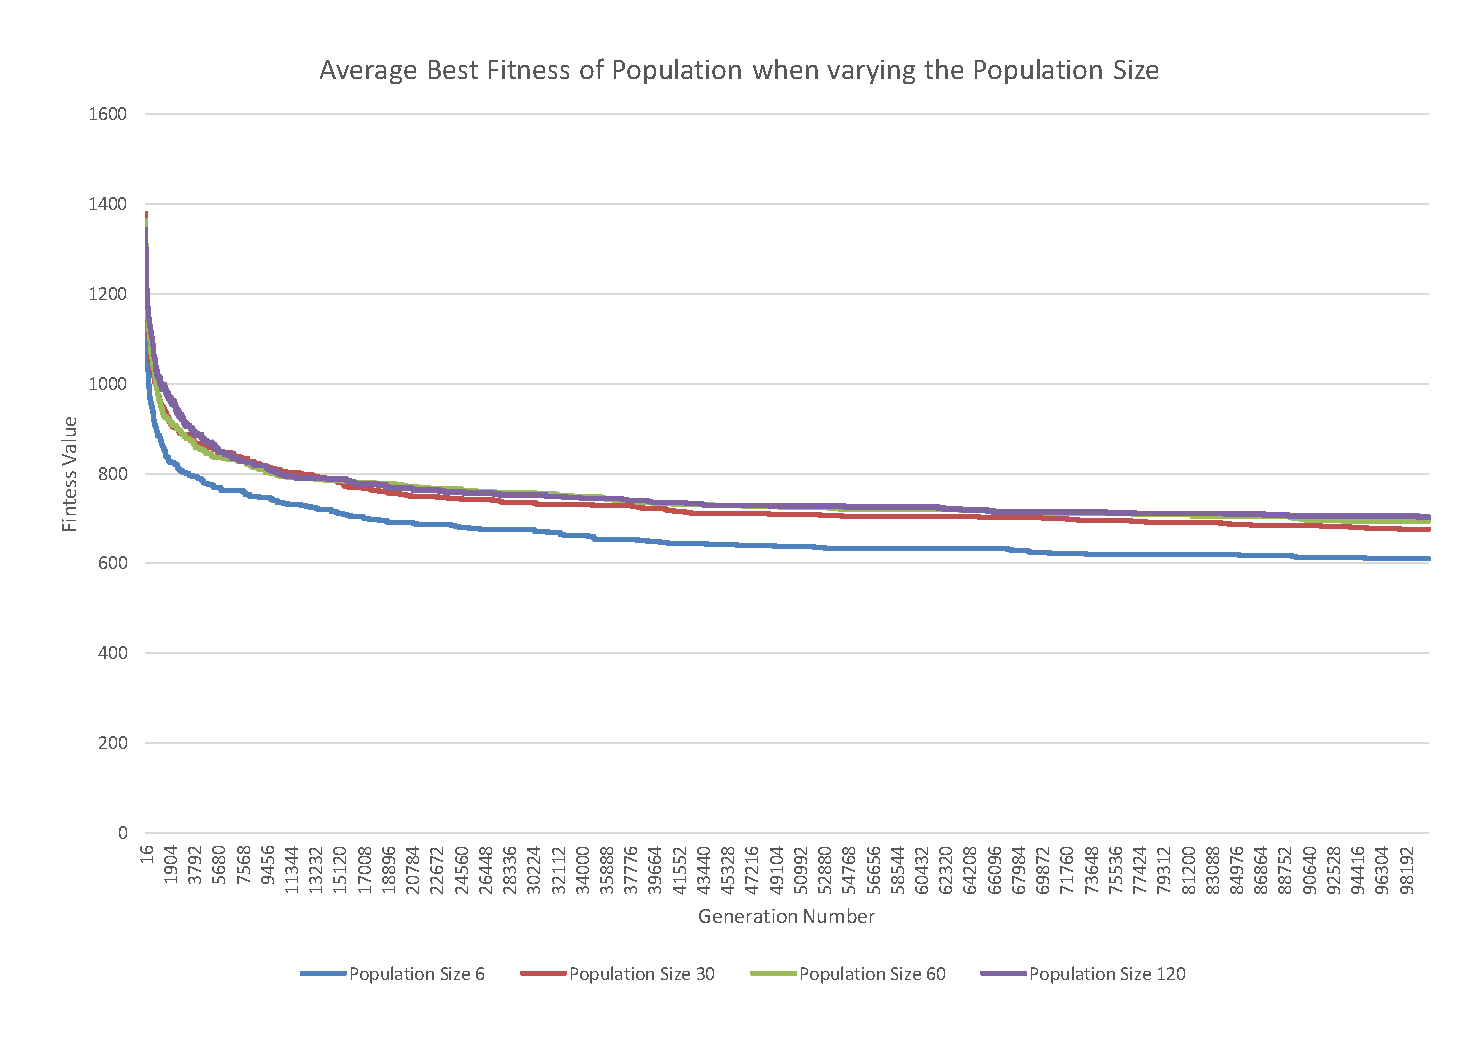
\includegraphics[width=\paperwidth]{figures/CircleTests/CircleTestsPopulationAverageBest.pdf}}
	\caption{//TODO - Average Best}
\end{figure}

\begin{figure}
	\centerline{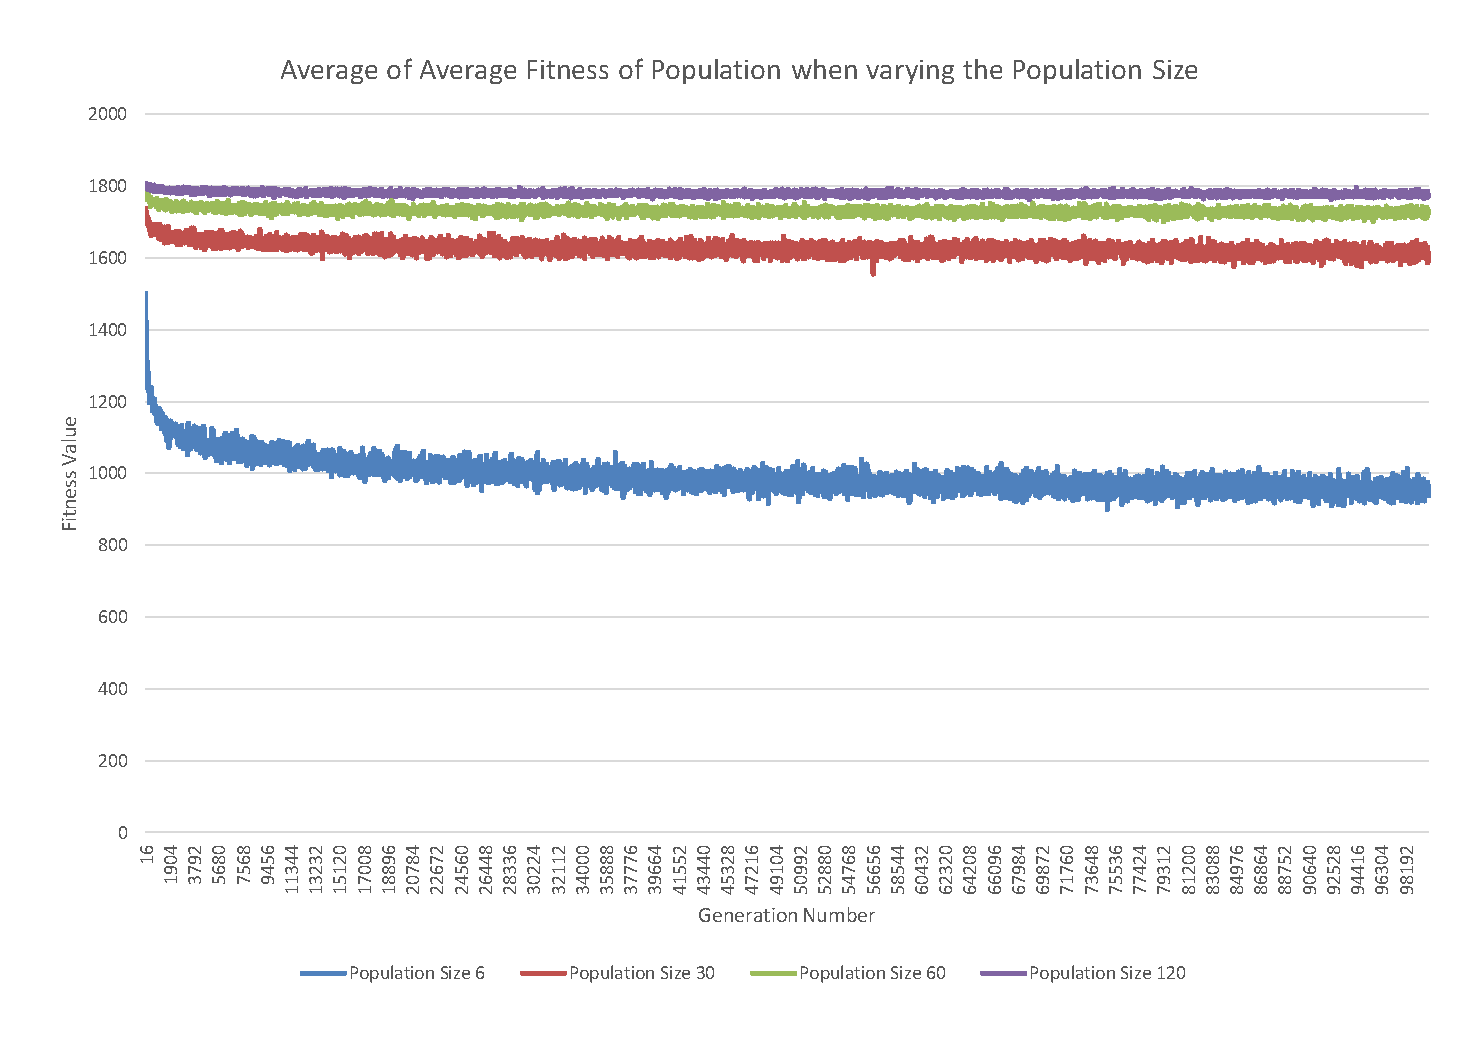
\includegraphics[width=\paperwidth]{figures/CircleTests/CircleTestsPopulationAverageAverage.pdf}}
	\caption{//TODO - Average Average}
\end{figure}

\begin{figure}
	\centerline{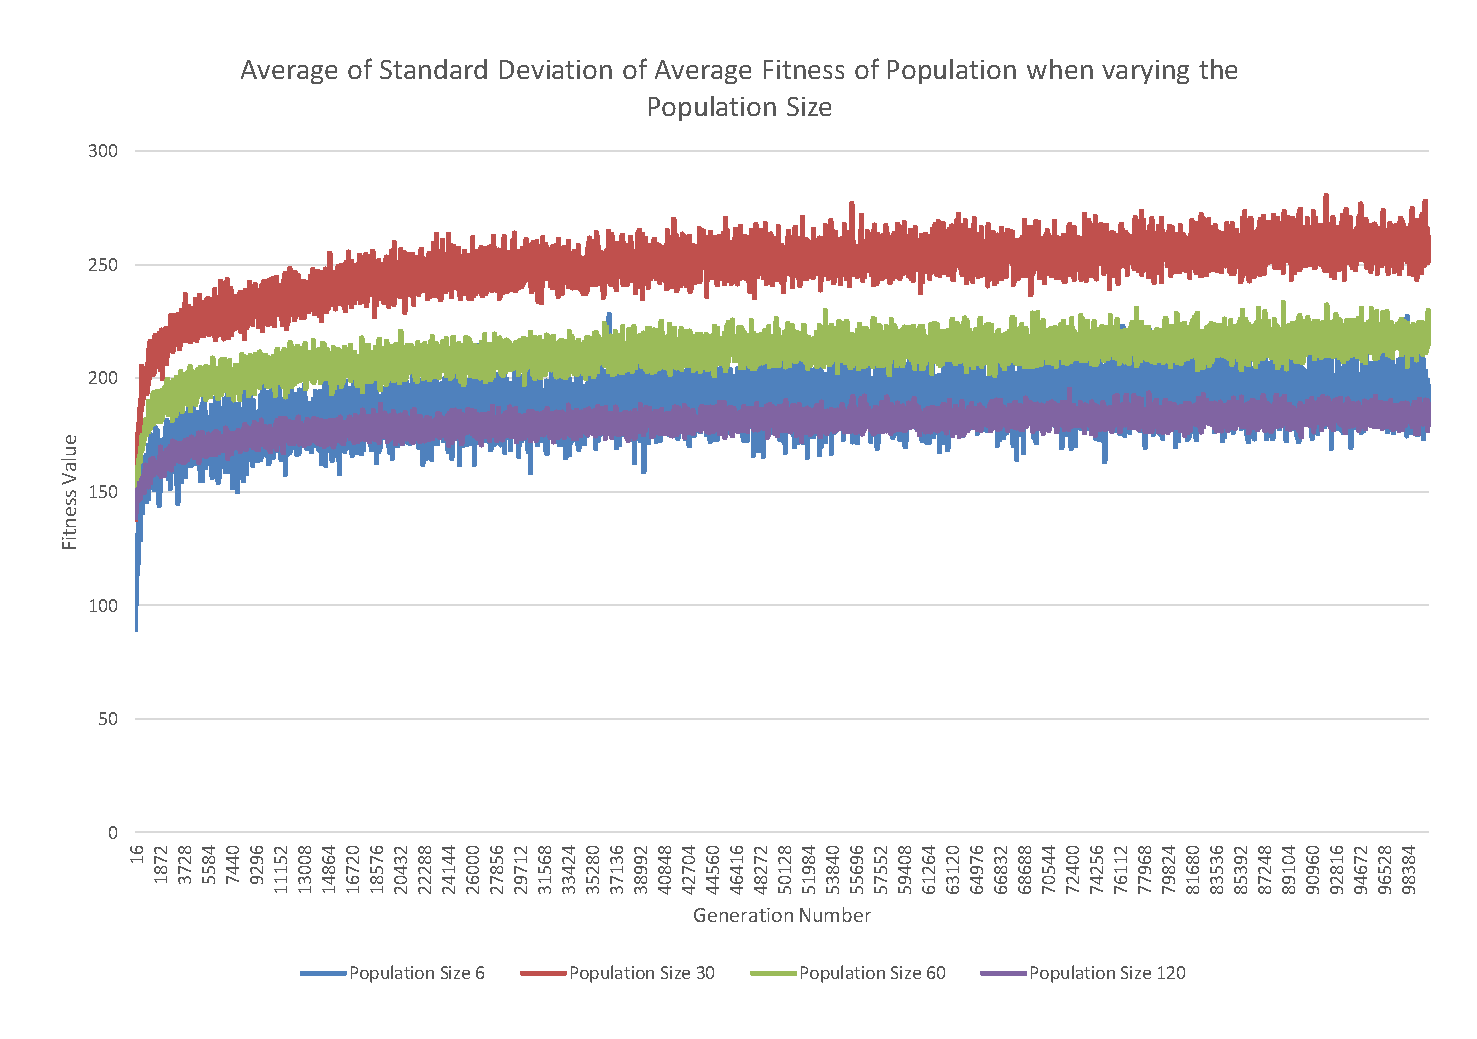
\includegraphics[width=\paperwidth]{figures/CircleTests/CircleTestsPopulationAverageStandardDeviation.pdf}}
	\caption{//TODO - Average Standard Deviation}
\end{figure}
% subsection Population Size (end)

\subsection{Parent Selection} % (fold)
\label{sub:parent_selection}
\begin{figure}
	\centerline{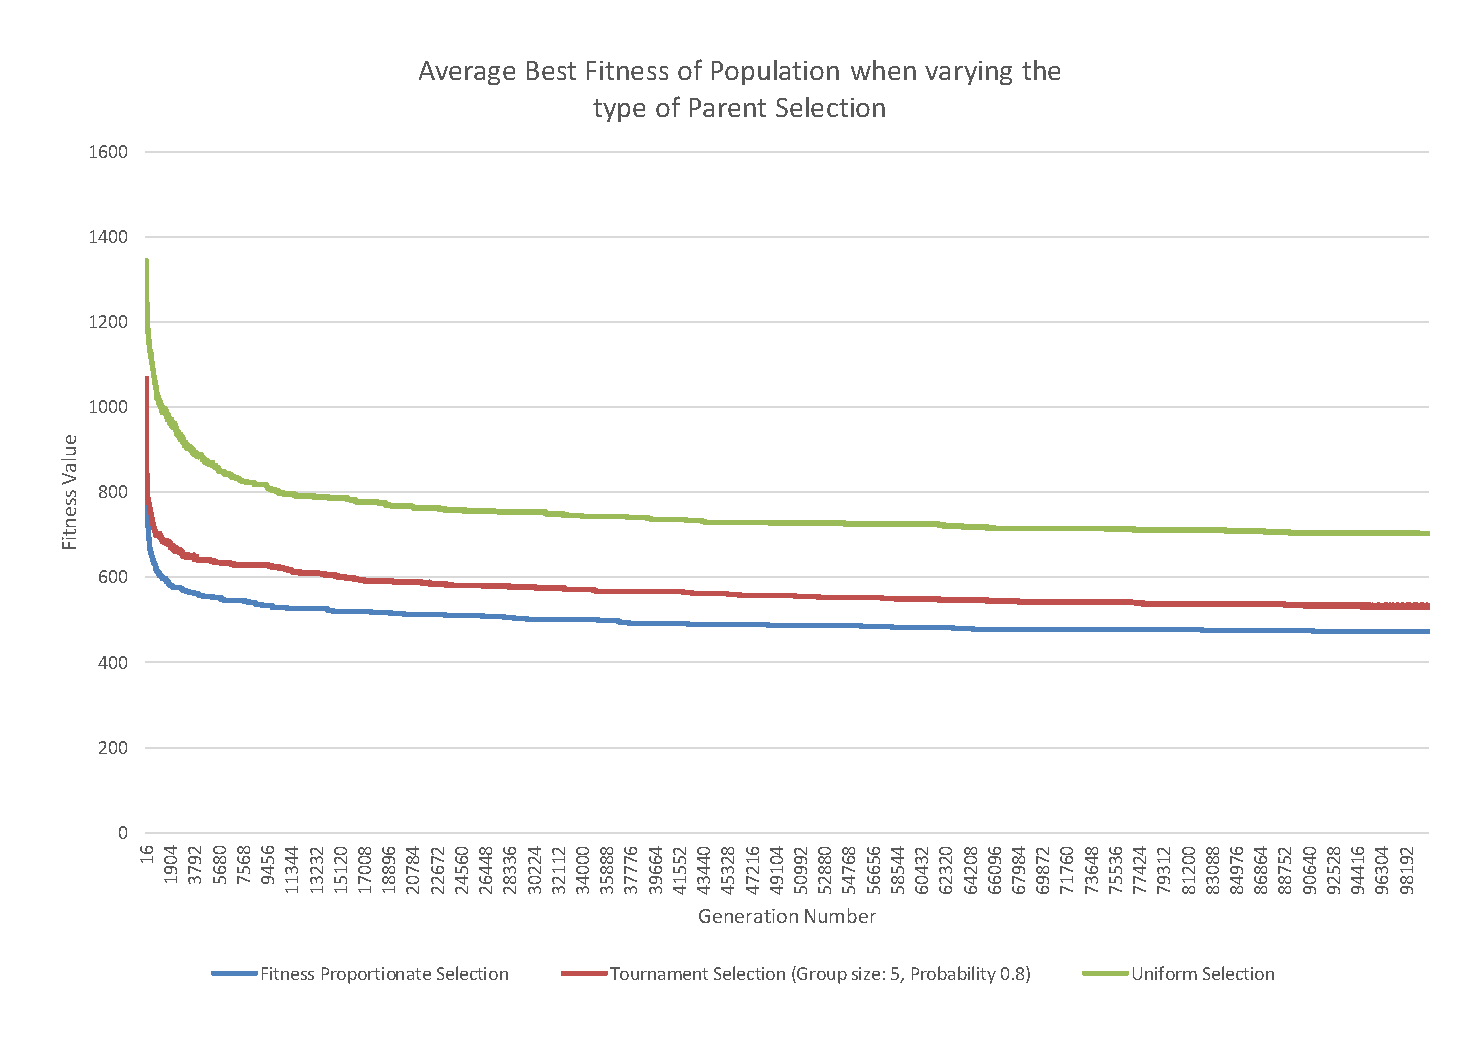
\includegraphics[width=\paperwidth]{figures/CircleTests/CircleTestParentSelectionAverageBest.pdf}}
	\caption{//TODO - Average Best}
\end{figure}

\begin{figure}
	\centerline{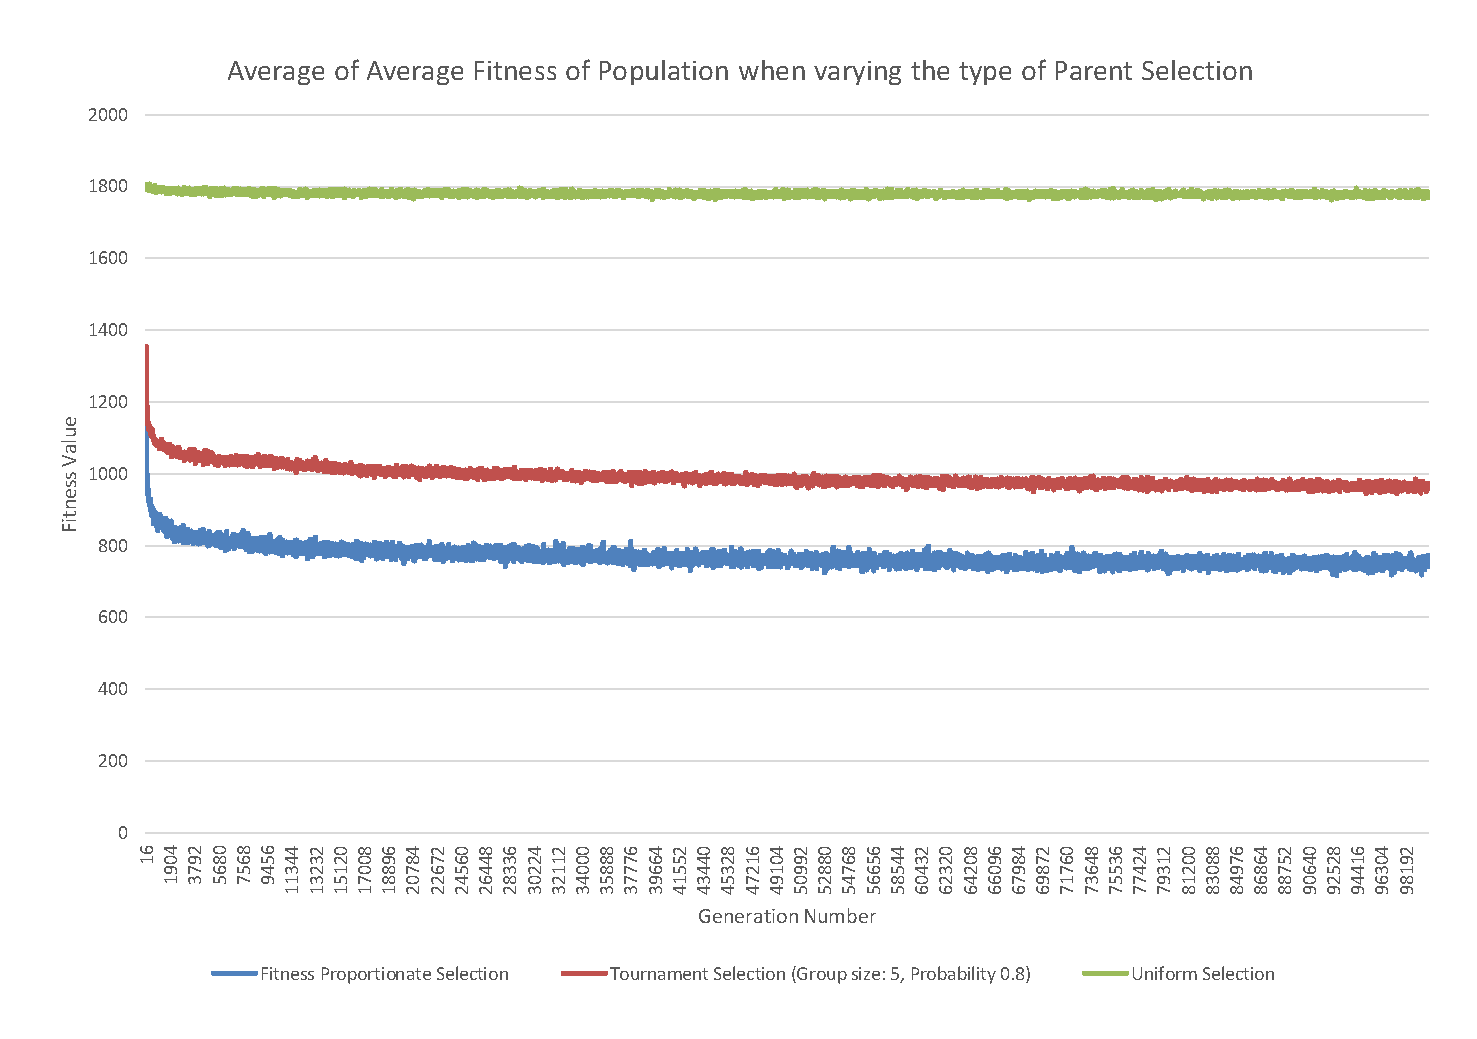
\includegraphics[width=\paperwidth]{figures/CircleTests/CircleTestParentSelectionAverageAverage.pdf}}
	\caption{//TODO - Average Average}
\end{figure}

\begin{figure}
	\centerline{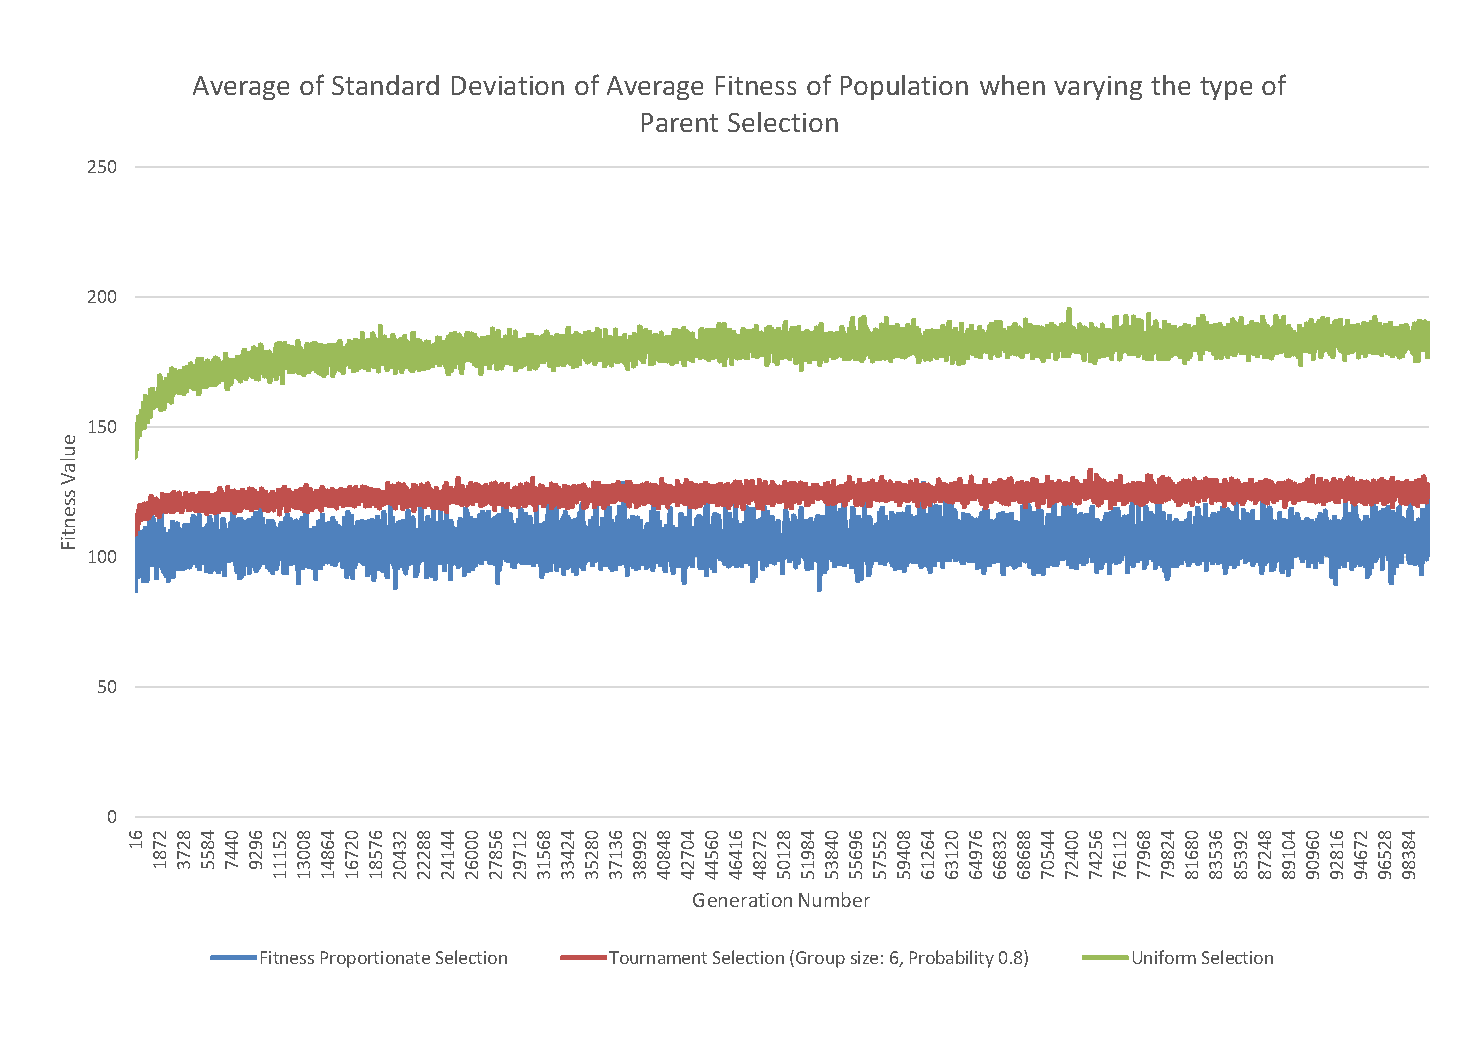
\includegraphics[width=\paperwidth]{figures/CircleTests/CircleTestParentSelectionAverageStandardDeviation.pdf}}
	\caption{//TODO - Average Standard Deviation}
\end{figure}
% subsection parent_selection (end)

\subsection{Adult Selection} % (fold)
\label{sub:adult_selection}
\begin{figure}
	\centerline{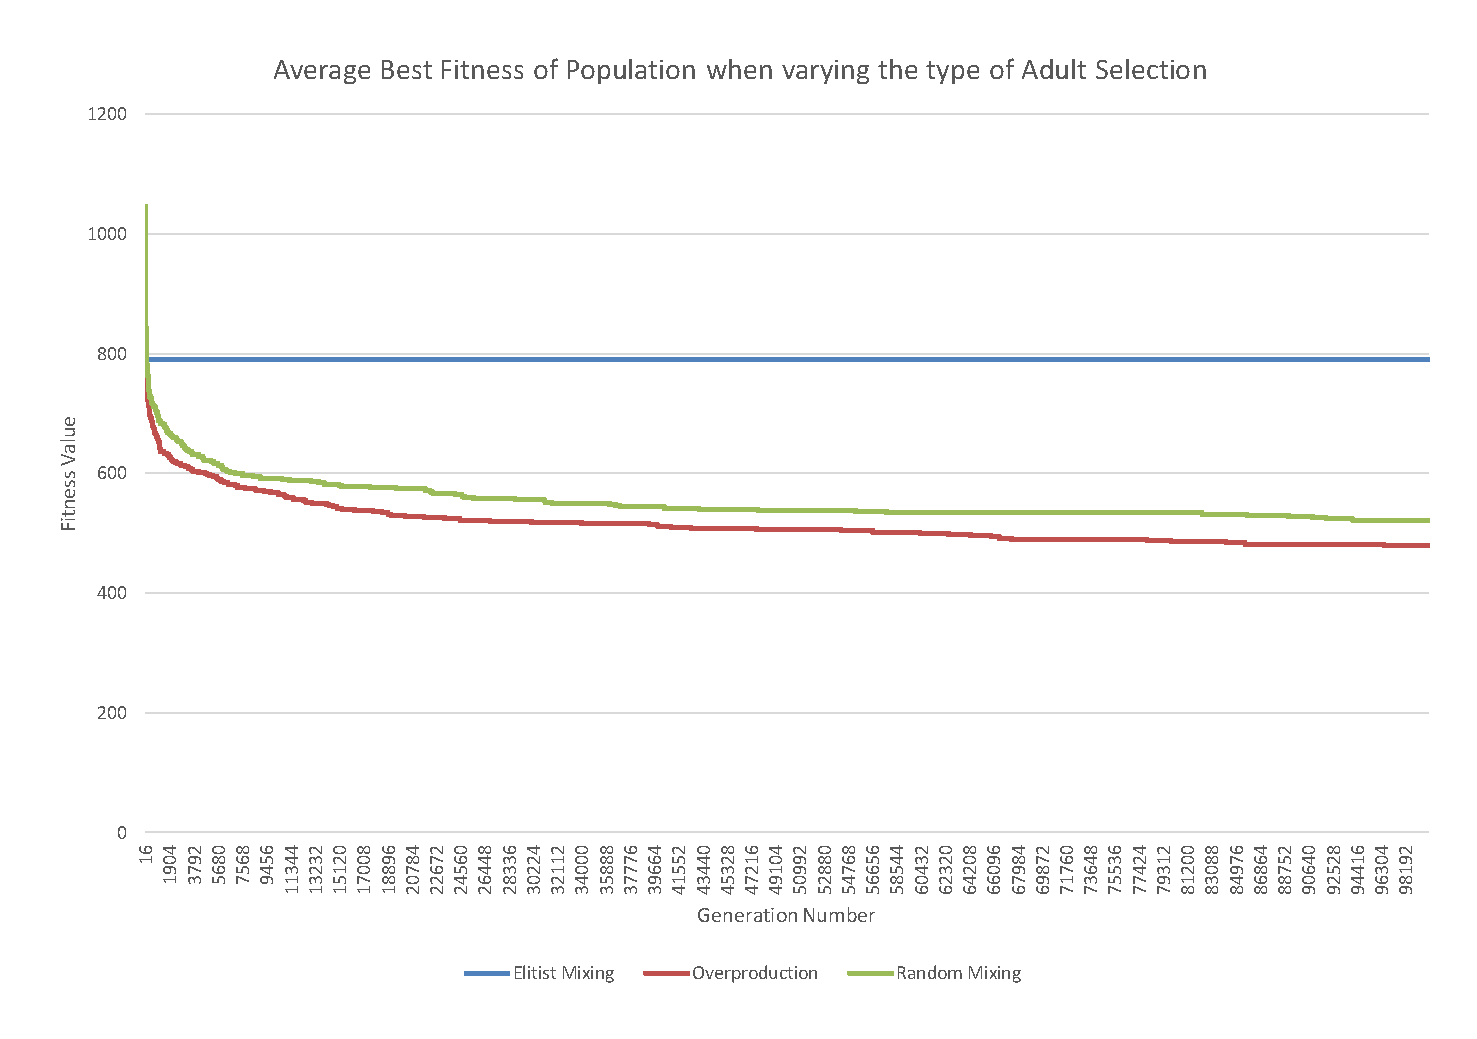
\includegraphics[width=\paperwidth]{figures/CircleTests/CircleTestAdultSelectionAverageBest.pdf}}
	\caption{//TODO - Average Best}
\end{figure}

\begin{figure}
	\centerline{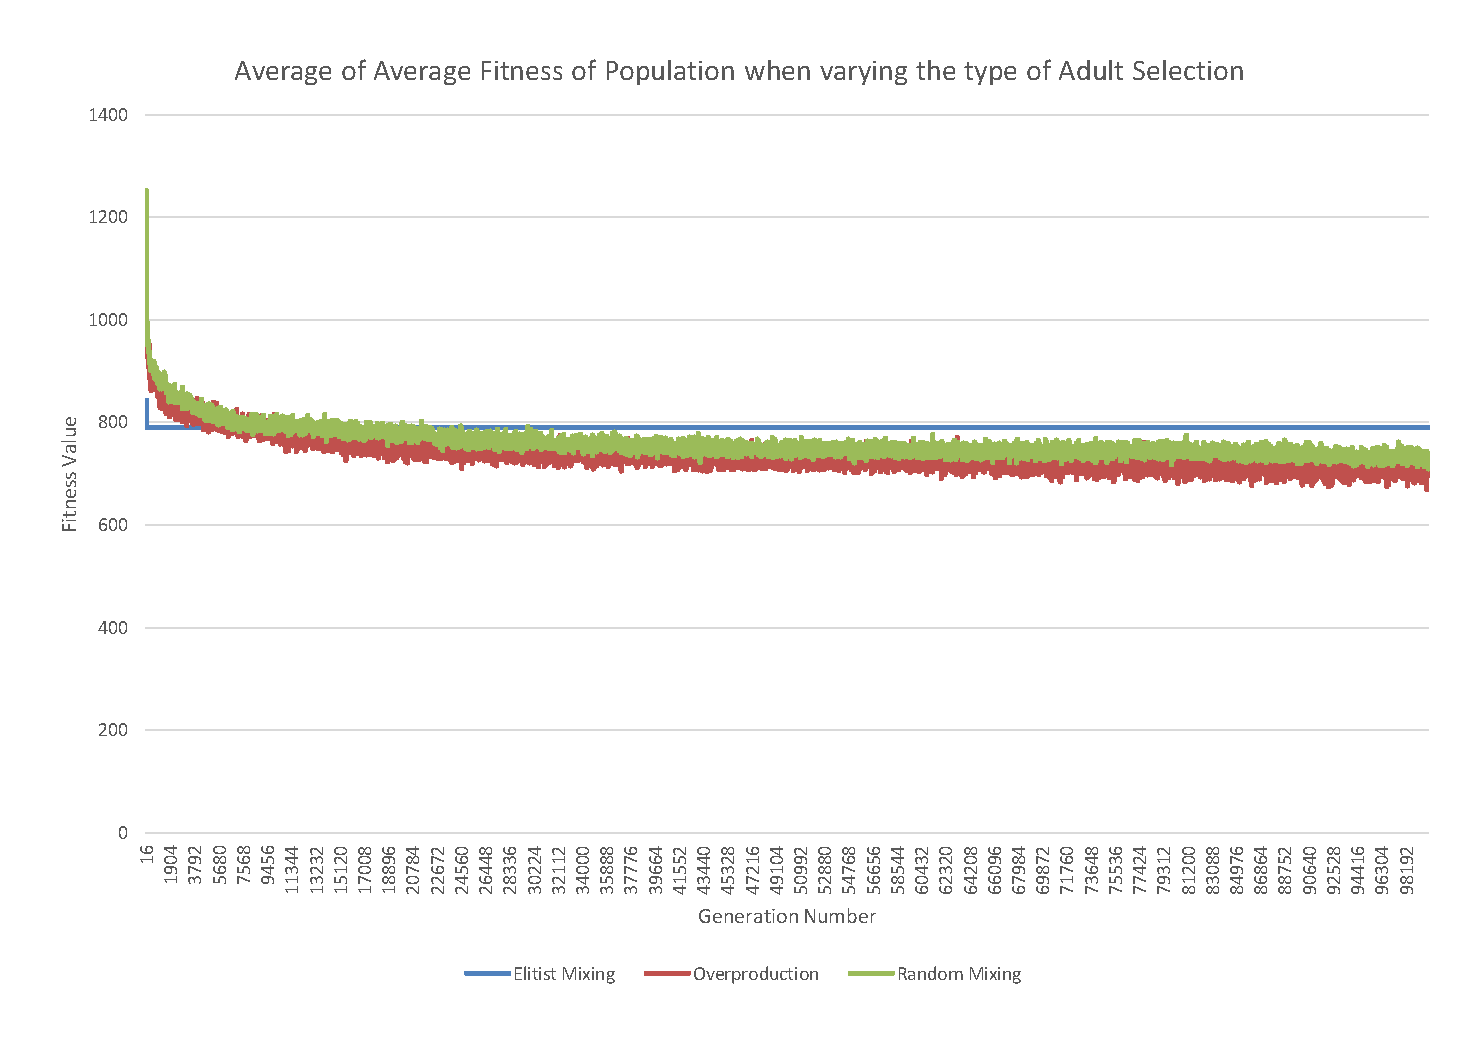
\includegraphics[width=\paperwidth]{figures/CircleTests/CircleTestAdultSelectionAverageAverage.pdf}}
	\caption{//TODO - Average Average}
\end{figure}

\begin{figure}
	\centerline{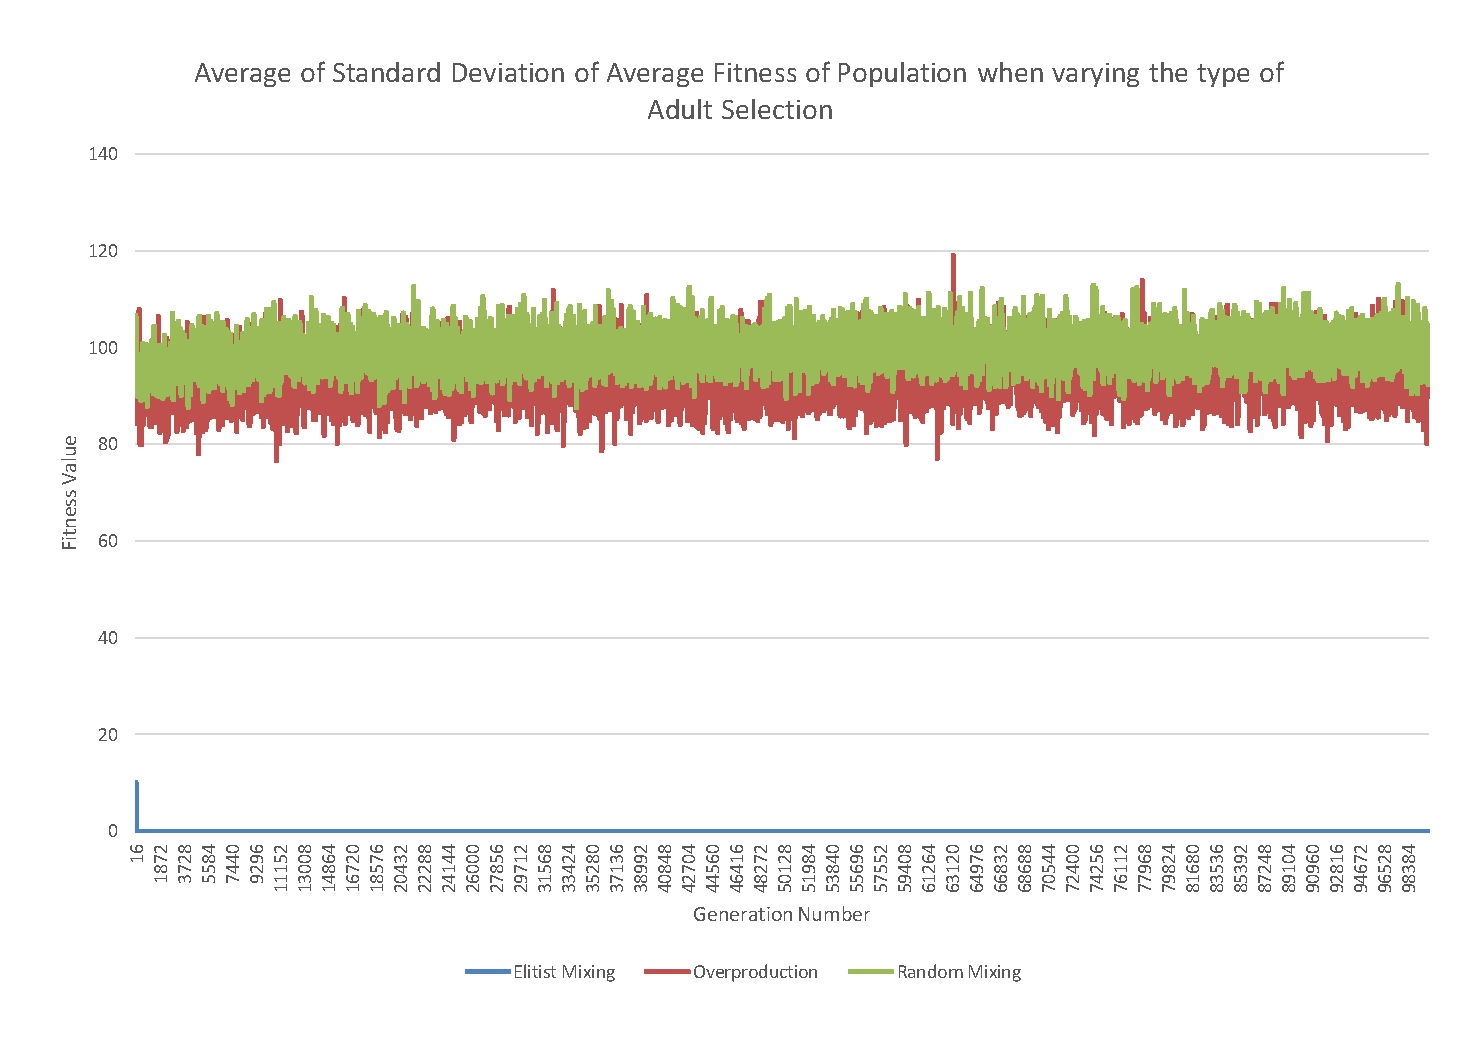
\includegraphics[width=\paperwidth]{figures/CircleTests/CircleTestAdultSelectionAverageStandardDeviation.pdf}}
	\caption{//TODO - Average Standard Deviation}
\end{figure}
% subsection adult_selection (end)

\subsection{Population Size Control} % (fold)
\label{sub:population_size_control}
\begin{figure}
	\centerline{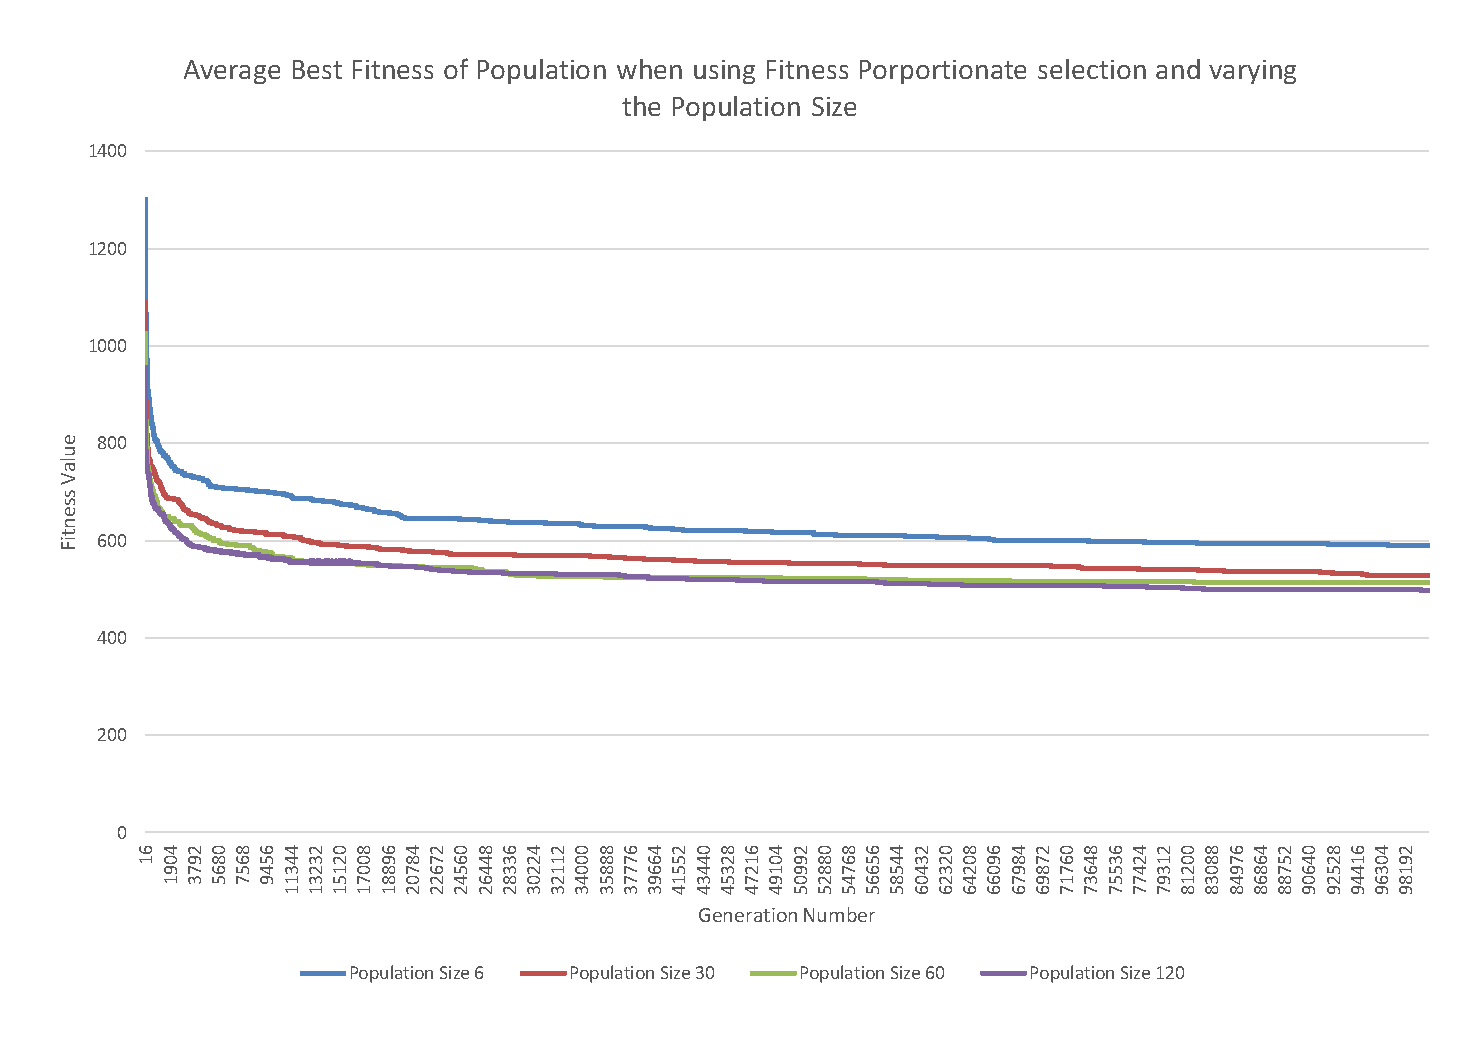
\includegraphics[width=\paperwidth]{figures/CircleTests/CirclePopulationSizeControllAverageBest.pdf}}
	\caption{//TODO - Average Best}
\end{figure}

\begin{figure}
	\centerline{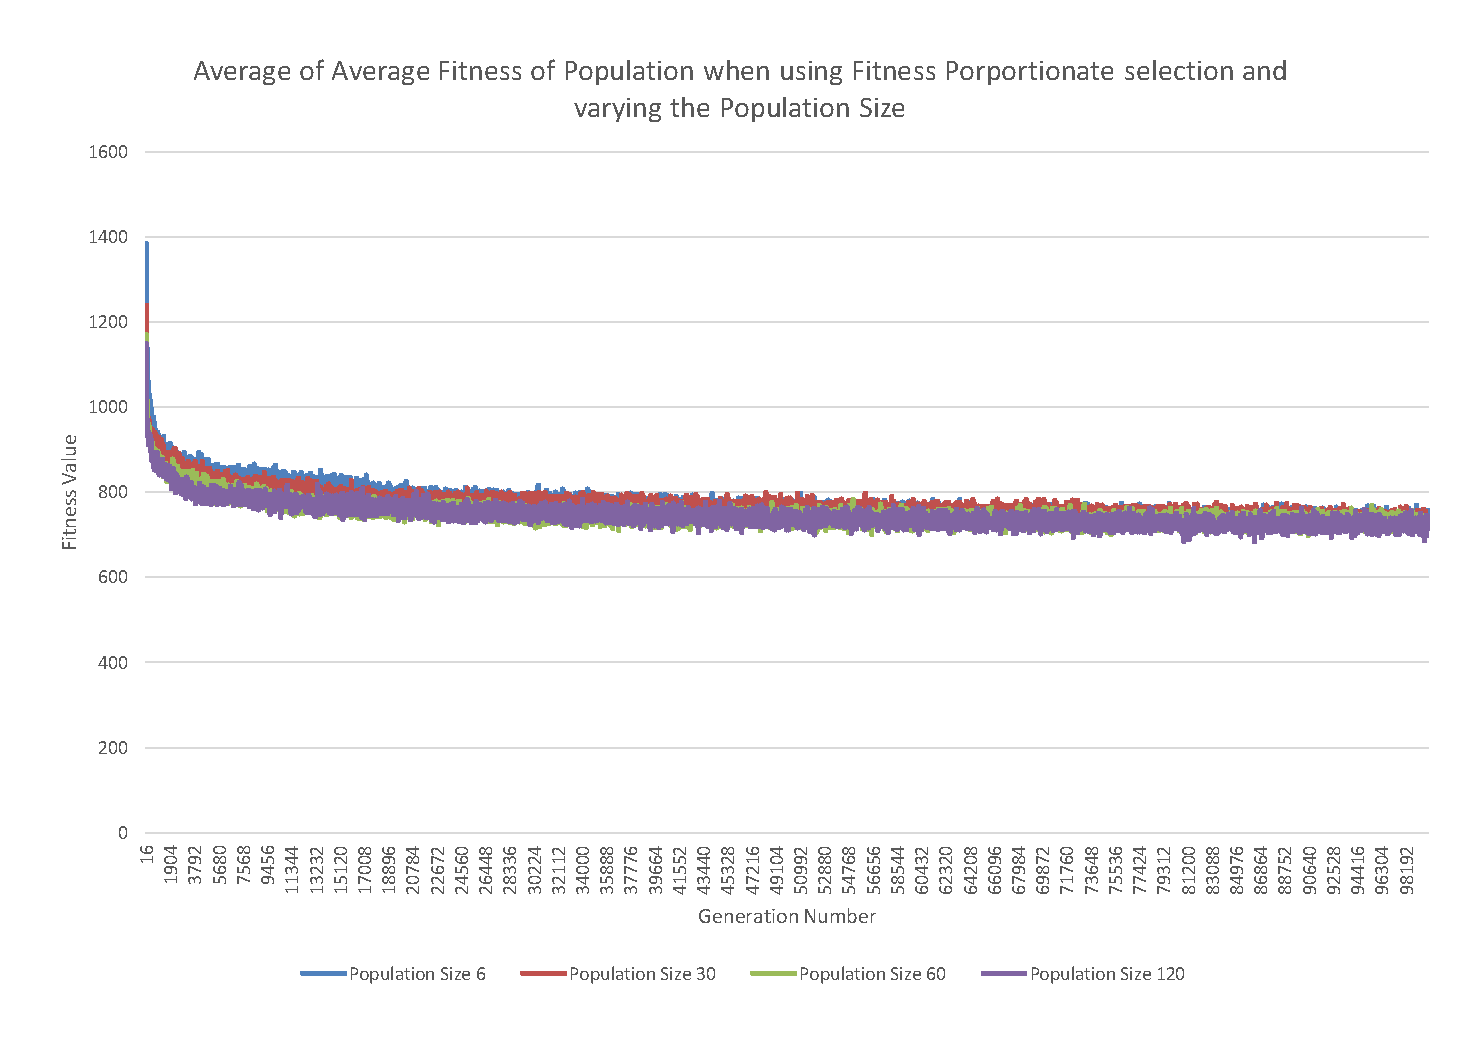
\includegraphics[width=\paperwidth]{figures/CircleTests/CirclePopulationSizeControllAverageAverage.pdf}}
	\caption{//TODO - Average Average}
\end{figure}

\begin{figure}
	\centerline{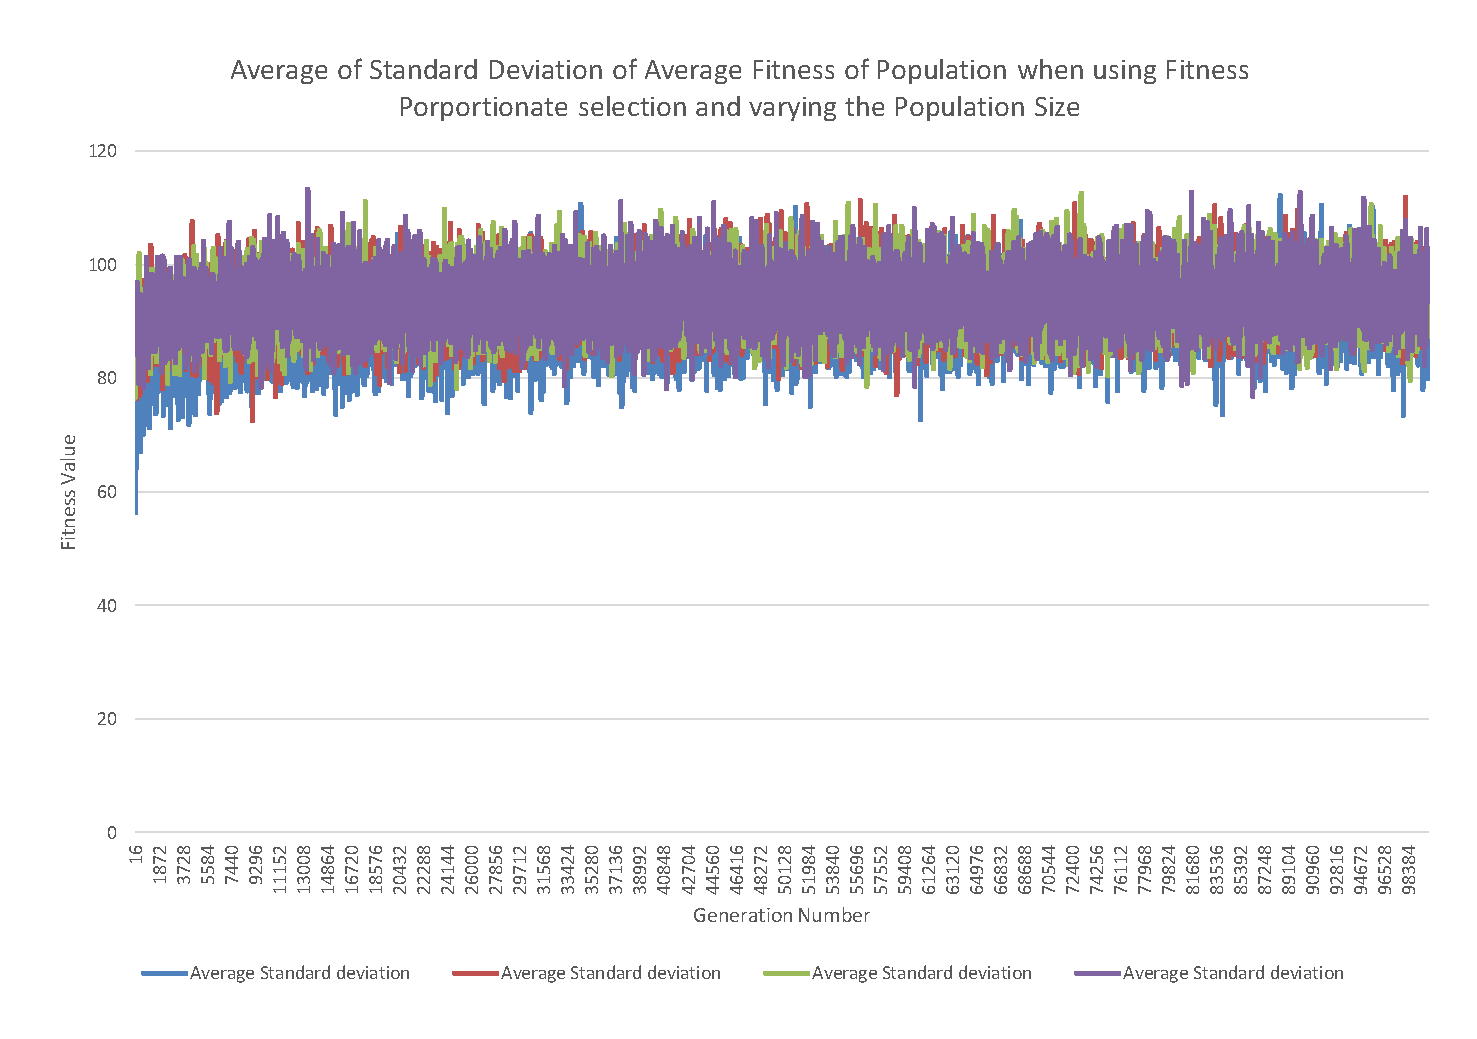
\includegraphics[width=\paperwidth]{figures/CircleTests/CirclePopulationSizeControllAverageStandardDeviation.pdf}}
	\caption{//TODO - Average Standard Deviation}
\end{figure}
% subsection population_size_control (end)


% section results (end)
\clearpage
\section{Evaluation and Conclusion} % (fold)
\label{sec:evaluation_and_conclusion}

% section evaluation_and_conclusion (end)

% chapter evolutionary_algorithm_configuration (end)